% Chapter 1: Introduction
\label{sec:introduction}

Deep learning has become a prominent solution in recent years for tackling image regocnision tasks. With the availability of large datasets, i.e. ImageNet, along with GPUs, training of deep learning models have become easier, and have led to remarkable results \cite{Goodfellow-et-al-2016}. The trained models have shown image classification with accuracies of over 80 \% \cite{he2015deepresiduallearningimage,dosovitskiy2021imageworth16x16words}, and hence the interest in deep learning for image recognition is high. However, the high accuracies are usually achieved on models trained with balanced datasets, while most real-world datasets are skewed in samples per class \cite{vanhorn2017deviltailsfinegrainedclassification,Buda_2018,liu2019largescalelongtailedrecognitionopen}.  

This thesis addresses the challenge of long-tailed datasets in image classification, where most classes contain only a few samples. A long-tailed class distribution causes the model to primarily learn features from majority (head) classes, leading to a bias toward these dominant classes. As a result, the trained model struggles to recognize inputs from minority (tail) classes. Most real-world datasets follows a long-tailed structure, hence the need for a reliable method to detect examples of tail-class data \cite{vanhorn2018inaturalistspeciesclassificationdetection,zhang2023deep}. The aim of this thesis is to examine class re-balancing techniques to tackle the long-tailed problem in deep learning.


\section{Problem Definition}
This thesis explores deep learning techniques for addressing long-tailed distributions in image classification, focusing on the interplay between backbone architectures and class-sensitive learning methods.

Four deep learning state-of-the art models are investigated, including three CNNs, and one ViT. The CNNs investigated are ResNet-50 \cite{he2015deepresiduallearningimage}, MobileNetV2 \cite{sandler2018mobilenetv2}, and ConvNeXt-Base \cite{liu2022convnet2020s}, while the ViT investigated is the ViT-B/16 \cite{dosovitskiy2021imageworth16x16words}. These particular models were chosen because of their individual strenghts  ResNet50 is a variant of the ResNet architecture, offering a strong baseline, providing a standard for comparison. MobileNetV2, build with the ResNet architecture, respresents models designed for environments with limited resources.ConvNeXt Base is a newer interpretation of convolutional neural networks, incorporating design principles from vision transformers, bridging the gap between tradional CNNs and ViTs, while ViT-B/16 represents traditional ViTs. All four models leverages transfer learning, pretrained on ImageNet \cite{ImageNet2009}, and subsequently trained on a balanced version of the CIFAR-100 \cite{krizhevsky2009learning} dataset, which serves as a baseline for comparing the training on the long-tailed version of CIFAR-100 (CIFAR-100-LT) \cite{cao2019learningimbalanceddatasetslabeldistributionaware}.  

The long-tailed techniques investigated in this thesis focus on class re-balancing, with an emphasis on class-sensitive learning through loss functions. All models are trained using Softmax Cross-Entropy Loss \cite{cs231n}, Weighted Softmax Cross-Entropy Loss \cite{zhang2023deep}, Focal Loss \cite{lin2018focallossdenseobject}, Class-Balanced Loss \cite{cui2019classbalancedlossbasedeffective}, Balanced Softmax Loss \cite{ren2020balancedmetasoftmaxlongtailedvisual}, LDAM Loss \cite{cao2019learningimbalanceddatasetslabeldistributionaware}, and Equalization Loss \cite{tan2020equalizationlosslongtailedobject}. By including these loss designs, this thesis investigates the effectiveness of each in mitigating the challenges posed by class imbalance.

The selection of these loss functions is based on their alignment with cost-sensitive approaches highlighted in Deep Long-Tailed Learning: A Survey \cite{zhang2023deep}. Starting with the standard Softmax Cross-Entropy Loss as a baseline, the study progresses through increasingly sophisticated loss functions designed to improve model performance on underrepresented tail classes while maintaining accuracy across the entire dataset. This comparative analysis aims to provide insights into how specific loss functions interact with model architectures in addressing the challenges of long-tailed distributions. 

By evaluating the effectiveness of different models and techniques, this study aims to guide practitioners in selecting appropriate strategies to address class imbalance, improve model performance on underrepresented classes, and achieve more balanced predictions.


\subsection{Goals of this thesis}
\label{sec:goals}
The goals of this thesis are to:

\begin{enumerate}
    \item Investigate the efficacy of long-tailed learning methods by assessing their performance on tail classes without sacrificing accuracy on head classes. 
    \item Understand how model design affects the performance of deep long-tailed learning methods.
    \item Provide a comprehensive insight in comparisons that inform the choice of methods for long-tailed distributions.
\end{enumerate}

\subsection{Hypothesis}
Deep long-tailed learning methods, such as the carefully designed loss functions tailored for long-tailed ditributed datasets, can improve the performance of underrepresented (tail) classes while maintaining the overall accuracy across diverse model architectures. The effectiveness of these loss functions is influenced by the choise of model architecture and the degree of imbalance of the dataset.


\subsection{Approach}
This master's thesis consists of five stages, described below:  
\vspace{1em}

\noindent \textbf{Stage one} is to investigate the dataset used for training, testing and validation in \textit{Deep Long-Tailed Learning: A Survey}, as the class re-balancing in this paper is used as inspiration for this thesis.
\vspace{1em}

\noindent \textbf{Stage two} is generating a long-tailed version of CIFAR-100 that can be used for training and comparisons of methods. This is inspired by Cao et al. \cite{cao2019learningimbalanceddatasetslabeldistributionaware}, who uses the CIFAR-100-LT dataset for experiments.
\vspace{1em}

\noindent \textbf{Stage three} is the selection of model architectures and class-sensitive methods.
\vspace{1em}

\noindent \textbf{Stage four} is training and evaluation of the models with different loss design. The training is both on the balanced and long-tailed versions of CIFAR-100.
\vspace{1em}

\noindent \textbf{Stage five} is a comparison of the methods.
\vspace{1em}



\subsection{Scope of this thesis}
This thesis seeks to apply deep long-tailed learning methods to image classification tasks with an emphasis on loss design to mitigate the effect imposed by class imbalance. The loss designs include Softmax Cross-Entropy Loss, Focal Loss, Weighted Softmax Cross-Entropy Loss, Class-Balanced Loss, Balanced Boftmax Loss, Equalization Loss, and LDAM Loss. The experiments are conducted on four backbone architectures: ResNet-50, MobileNetV2, ConvNeXt-Base, and ViT-B/16. These are trained on the CIFAR-100 dataset with both a balanced and synthetically generated long-tailed version. The evaluation metric is the top-1 accuracy, with attention paid to performance on head, middle, and tail classes. This thesis does not explore other long-tailed learning approaches such as re-sampling, information augmentation, or model architecture modifications.




\section{Related Work}
The challenge of long-tailed datasets has been extensively studied in the literature \cite{zhang2023deep,zhang2024systematicreviewlongtailedlearning}, and to overcome the challenge of long-tailed data, various methods has been proposed. Zhang et al. \cite{zhang2023deep} conducted a comprehensive survey on long-tailed learning techniques, categorizing them into three main strategies: class re-balancing, information augmentation, and module improvement. These are further divided into sub-categories: re-sampling, cost-sensitive learning, logit adjustment, transfer learning, data augmentation, representation learning, classifier design, decoupled training, and ensemble learning, as seen in Figure~\ref{fig:lt_methods}. 

This section highlights methods relevant to the experiments conducted in this thesis; for additional details on other techniques, refer to the references cited in Zhang et al.'s survey.

\begin{figure}[ht]
    \centering
    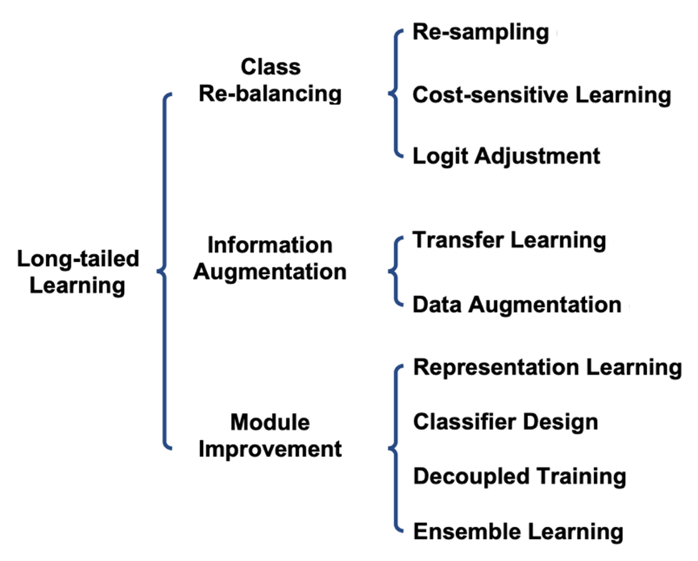
\includegraphics[width=0.8\textwidth]{Images/lt_methods_categories.png} 
    \caption{Proposed categorization of long-tailed methods by \emph{Zhang et al.} \cite{zhang2023deep}. There are three main categories: class re-balancing, information augmentation, and module improvement. These are further divided into sub-categories: re-sampling, cost-sensitive learning, logit adjustment, transfer learning, data augmentation, representation learning, classifier design, decoupled training, and ensemble learning.}
    \label{fig:lt_methods} 
\end{figure}


\paragraph{Data Re-sampling}
Data re-sampling techniques aim to modify the training dataset to mitigate class imbalance by simulating a balanced dataset. The most popular methods for re-sampling are random over-sampling (ROS) and random under-sampling (RUS) \cite{Chawla_2002}. ROS involves duplicating random samples from the minority classes, whereas RUS involves removing samples from the majority classes \cite{zhang2023deep}. However, these techniques have their weaknesses: over-sampling the minority classes will eventually lead to overfitting tail classes, and under-sampling can lead to underperformance on head classes \cite{zhang2023deep}. Another re-sampling technique, called Synthetic Minority Over-Sampling Technique (SMOTE) \cite{Chawla_2002}, involves synthetical generation of instances of the minority classes based on the existing data. 

\paragraph{Re-weighting}
Re-weighting techniques attemps to address class imbalance by assigning weights to classes or samples during training. The vanilla approach involves weighting classes proportional to the inverse sample frequency \cite{zhang2023deep}. Cui et al. \cite{cui2019classbalancedlossbasedeffective} propose re-weighting by the inverse effective number of samples. Focal Loss \cite{lin2018focallossdenseobject} introduces a mechanism to down-weight well-classified examples, emphasizing harder examples during training. Tan et al. \cite{tan2020equalizationlosslongtailedobject} proposed down-weighting tail-class loss when they serve as negative vaules for head-classes. These re-weighting strategies form the foundation for comparison in this thesis.

\paragraph{Margin}
Margin-based approaches aim to improve classification performance by increasing the separation between classes. Techniques such as Large-Margin Softmax \cite{liu2017largemarginsoftmaxlossconvolutional} and Additive Margin Softmax \cite{Wang_2018} reduce intra-class variation and enhance inter-class separability.

Label-Distribution-Aware-Margin (LDAM) Loss \cite{cao2019learningimbalanceddatasetslabeldistributionaware} focuses on integrating margin-based strategies with class-sensitive learning to explicitly encourage larger margins for tail classes. The performance of this re-margining strategy is evaluated in this thesis.

\paragraph{Logit Adjustment}
Logit adjustment methods seeks to modify the prediction logits of deep models, either applied post-hoc to a trained model, or enforced during training \cite{menon2021longtaillearninglogitadjustment}. Balanced Softmax Loss \cite{ren2020balancedmetasoftmaxlongtailedvisual} adjusts logits by incorporating class priors into the Softmax function, ensuring a more stable probability assignment across classes. The performane of the Balanced Softmax Loss is evaluated in this thesis.

\paragraph{Transfer Learning}
Transfer learning techniques adress the issue of class imblance by transferring learned features from head classes to tail classes. Examples include transferring the intra-class variance \cite{yin2019featuretransferlearningdeep} and transferring semantic deep features \cite{liu2019largescalelongtailedrecognitionopen}.

\paragraph{Data Augmentation}
Data augmentation is a deep learning technique used to expand the training dataset by applying transformations to samples or features, enhancing model accuracy while reducing overfitting \cite{perez2017effectivenessdataaugmentationimage,shorten2019survey}. Common augmentation methods include Mixup \cite{zhang2018mixupempiricalriskminimization}, which combines pairs of samples to create interpolated examples, CutMix \cite{yun2019cutmixregularizationstrategytrain}, which replaces regions of one image with patches from another, and UniMix \cite{xu2021calibratedmodellongtailedvisual}, which focuses on calibrating the feature space for long-tailed distributions. Rare-class Sample Generator (RSG) \cite{wang2021rsgsimpleeffectivemodule} focuses on enhancing tail-class performance by transferring knowledge from head classes.


\paragraph{Ensemple Learning}
Ensemble learning is a technique that combines multiple network modules (i.e. experts) to solve long-tailed problems. By doing so, the predictions of the different models can be combined, ultimately outperforming a single model \cite{zhou2020bbnbilateralbranchnetworkcumulative,wang2022longtailedrecognitionroutingdiverse}.

% \paragraph{Decoupled Training}
% Decoupled training \cite{kang2020decouplingrepresentationclassifierlongtailed} separates representation learning and classifier training. First, the model is trained to extract features from the entire dataset, afterwards, a re-balancing technique is applied during classification. Despite the simple framework, decoupling showed state-of-the art performance on long-tailed benchmarks.


\section{Reading Guide}

\noindent \textbf{Structure} This reading recommendation is to read this thesis in a linear flow, beginning with Chapter 1 followed by Chapter 2 etc. However, if the reader is familiar with the subjects of this thesis, Chapter 2 can be skipped, and the reader can go to Chaper 3. Alternatively, if the reader is familar with long-tailed methods and looking for a quick guidance, jumping directly to Chapter 5 will suffice, although it is highly recommended to read Chapter 4 for a better understanding of Chapter 5.
A description of the content of the chapters is presented in the following:
\vspace{1em}

\noindent \textbf{Chapter 2} provides the theoretical background for the long-tailed learning methodologies relevant to the work in this thesis.
\vspace{1em}

\noindent \textbf{Chapter 3} describes the methodology used in this thesis, including dataset preparation, selection of model and loss designs, and implementation details. 
\vspace{1em}

\noindent \textbf{Chapter 4} present the experimental results and a discussion thereof.
\vspace{1em}

\noindent \textbf{Chapter 5} concludes on this thesis, reflects the goals presented in Chapter 1, and discusses future work. 

